\chapter{Evaluation of the concept}
For the evaluation of the results obtained from the work, we proceed in two steps. First is the analysis of Raycasted point cloud and second is the analysis of casted shadow. For the evaluation of raycasted point cloud, a scatter plot is created. The distance of the prototype is varied in the target scene cloud from the origin and raycasted point cloud was calculated. This graph proves that the number of raycasted points in the point cloud of the prototype surface increases when moving towards the origin and the number of point cloud points decreases as moving away from the origin. A 3d plot between the original prototype and the raycasted prototype point cloud is plotted. The raycasted prototype is obtained without transforming the prototype location. This graph is created to show the difference between the original prototype points and the raycasted prototype points by visualizing them in 3d plots. Overlapping points in both the point clouds in the 3d plot graph verifies their similar nature. A graph plotting the distance between the corresponding points between the original prototype cloud and the raycasted prototype cloud is plotted. This graph shows that points that are considered equivalent between the two point clouds have a very low distance gap. Geometric feature distribution is plotted for the two point clouds (original prototype point cloud and raycasted prototype point cloud) with equivalent parameters to show the similarity in geometric features (surface variation).

For the evaluation of the predicted shadow, two point clouds are captured where the only difference between the two point clouds is the availability of a prototype (person). One point cloud consists of a person and its casted shadow, we call this a source scene cloud. Another point cloud does not consist of the same person or its shadow but the background information or all the other points in the point cloud is similar. We call this point cloud target scene cloud. A prototype (person) point cloud is extracted from the source scene cloud and inserted into the target scene cloud without transformation. The shadow cast by the prototype on the target scene cloud is computed. To evaluate the precision of the predicted shadow, a confusion matrix was created. Equivalent points between the two point clouds were searched in a selected region on both point clouds. Using the nearest neighbor search, equivalent points were computed. The confusion matrix shows that maximum points were similar on both the point clouds. The validity of the equivalent points is shown by creating a plot that shows the distance between the points in the predicted shadow cloud and their equivalent points in the original shadow cloud ( equivalent points computed for a bounded region that covers the shadow cast region by the person). The low difference between the equivalent points, in the order of \(1e-9\), shows the validity of the confusion matrix plot. IOU between the predicted shadow and ground truth shadow region is computed. This verifies that the shadow casted by the prototype is accurately predicted. The area of the predicted shadow was more in comparison with the ground truth shadow because the reconstructed surface for the prototype (person) had a bigger surface area than the actual prototype.

\section{Evaluation of Raycasted Pointcloud}
A raycasted point cloud is the point cloud that is obtained after projecting rays from the origin to the surface of the prototype after reconstructing the surface into triangular meshes. Methods like calculation of average distance, comparing the number of points, and comparing the vanilla 3D points were used for the evaluation of raycasted point cloud. These methods are discussed below.
\subsection{Average distance from the origin vs number of points}
With this step, we check the variation of the number of points in the raycasted point cloud when changing the position of the prototype before raycasting concerning origin. The distance between the prototype cloud and the origin of the target scene point cloud was changed by transforming the extracted prototype to a different location on the target cloud. The distance from a prototype to the origin is calculated by calculating the Euclidean distance from the origin to each point in the prototype. The average was obtained after dividing the sum of the distances of each point in the prototype by the number of points. Rays were cast to the surface of the prototype after surface reconstruction.  Change in points number based on different locations of the transformed prototype on the target scene cloud is observed.

\begin{figure}[htbp]
    \centering
    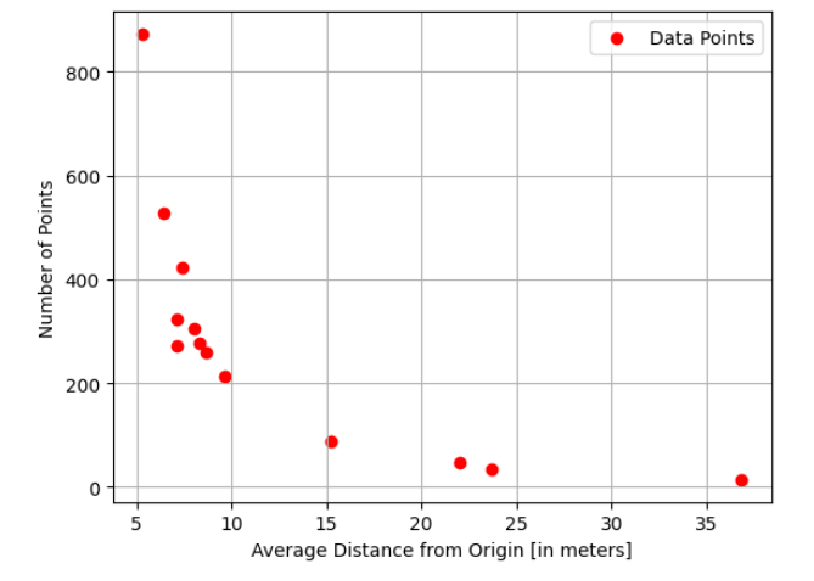
\includegraphics[width=0.8\linewidth]{97_graphics/evaluation/avg_distn_vs_points_numbers.pdf}
    \caption{Averge distance from the origin [in meters] vs Number of points in Raycasted Point cloud}
    \label{fig:evalution_avg_distn_vs_points_number}
\end{figure}
In this figure \ref{fig:evalution_avg_distn_vs_points_number}, the original prototype is positioned at about 7 meters from the origin. The prototype was moved closer toward the origin and farther away from the origin on the target cloud, and the raycasted point cloud of the prototype was calculated. From the graph, as shown in figure \ref{fig:evalution_avg_distn_vs_points_number}, it can be seen that the number of points on the raycasted prototype decreases after an increase in the average distance between the prototype and the origin. The number of points of the raycasted prototype increases on decreasing the distance from the origin.

\subsection{3D plot of the original and raycasted prototype}\label{sec:3dplot}
To visualize the similarities between the corresponding points on the original and raycasted prototype point cloud, a simple 3D plot in the XYZ axis can be analyzed. For this evaluation, the difference between the original prototype and the raycasted prototype is shown where the raycasting was done without varying the position of the prototype on the target cloud.

\begin{figure}[htbp]
    \centering
    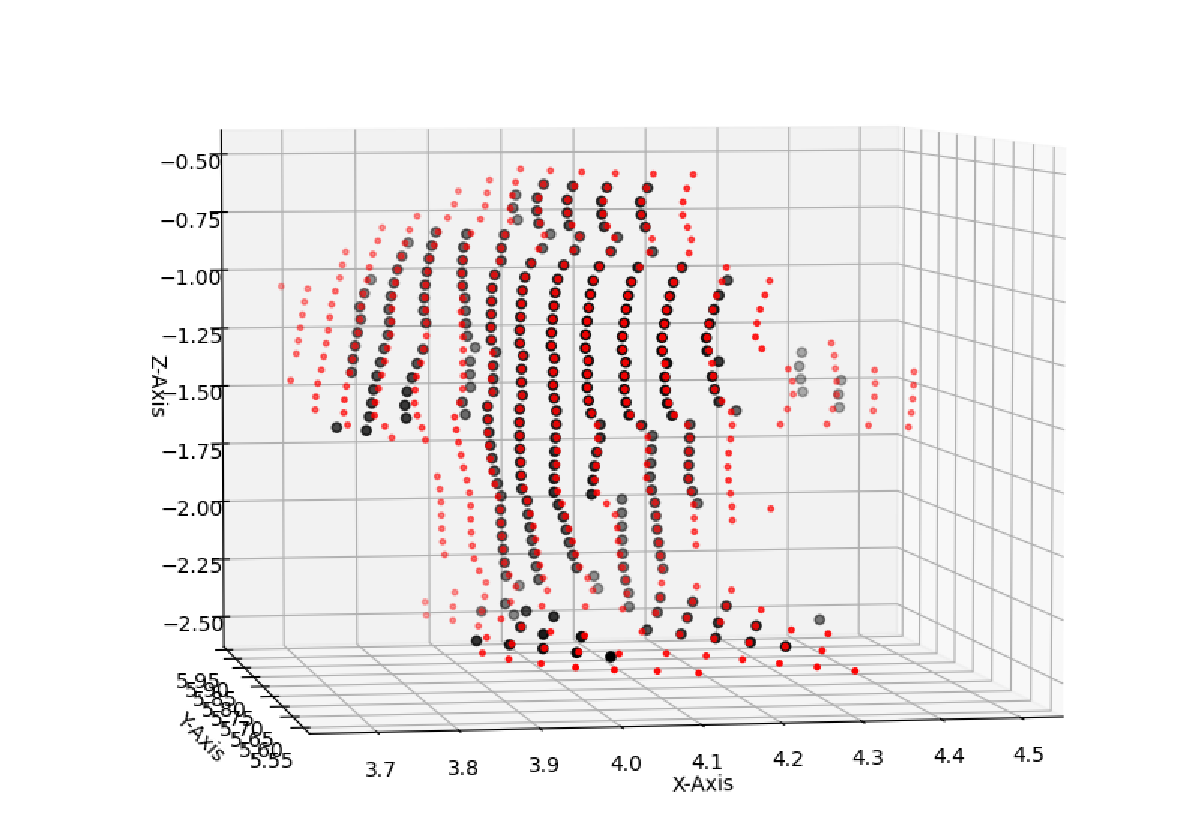
\includegraphics[width=1\linewidth]{97_graphics/evaluation/3dxyz_plot.pdf}
    \caption{3D XYZ Plot}
    \label{fig:evaluation_3dplot}
\end{figure}

The graph can be viewed in figure \ref{fig:evaluation_3dplot}. The black points in the graph correspond to the point in the prototype before raycasting. The red points in the graph correspond to the point of the prototype after raycasting. It can be observed that most of the red points overlap the black points, which proves that there is a low difference between the original prototype and the prototype cloud after raycasting. Most of the red points that do not overlap with the black points are due to the bigger area of the reconstructed surface. Proper filtering of the reconstructed surface would result in the removal of the red outliers.

\subsection{Distance between the corresponding points}
Distance between the corresponding points was calculated between the original prototype cloud and the prototype cloud after raycasting. The raycasting was performed on the original prototype surface without transformation. We calculated the average distance between the black points and the corresponding red points of the figure \ref{fig:evaluation_3dplot}. To find the corresponding points between two clouds, spheres with different values of radius were experimented for the calculation of the nearest neighbor. Neighbors for a point in the original prototype were calculated from the raycasted point cloud that falls within the radius of the sphere. The neighbor that has the minimum distance from the ego point was chosen. This point in the raycasted prototype is considered the equivalent point of the ego point in the original prototype. Sphere size can be lower or higher for neighbor search. This is because whatever the size of the sphere, we are extracting a point from the sphere that has the least distance from the ego point/ center of the sphere. However, too low value for radius might lead to not finding any neighbors.
\begin{figure}[htbp]
    \centering
    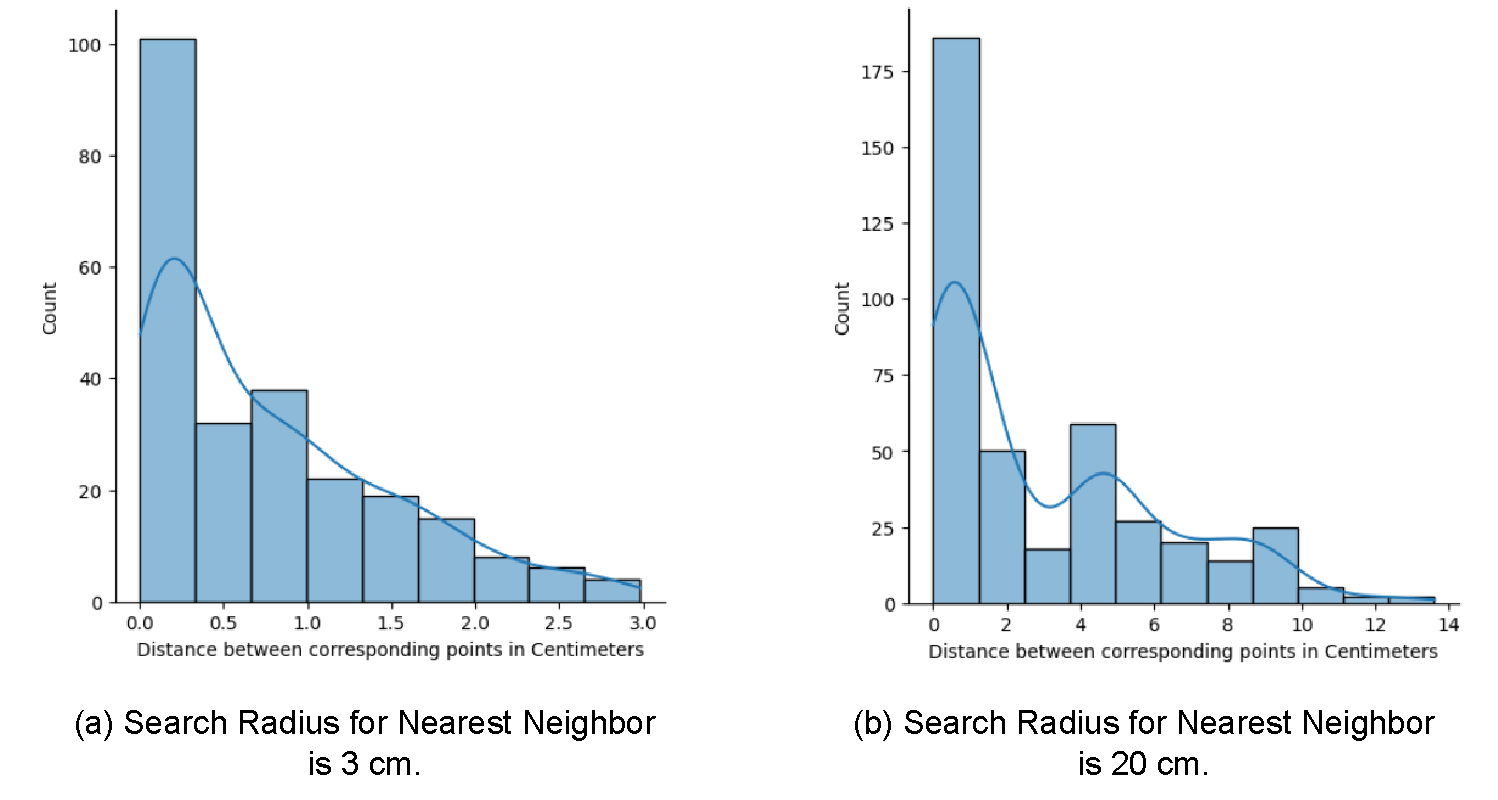
\includegraphics[width=1\linewidth]{97_graphics/evaluation/distn_betn_corresponding_points_in_raycasting.pdf}
    \caption{Distance between the corresponding points in centimeters}
    \label{fig:evaluation_distn_corresponding_points}
\end{figure}
Figure \ref{fig:evaluation_distn_corresponding_points} shows plots of the distance between the black points and their equivalent red points from figure \ref{fig:evaluation_3dplot}. Figure (a) is plotted after finding the nearest neighbor with a search within the sphere of radius 3 cm centered around an ego point. When searching the neighbor with 3cm, out of 408 points in the raycasted point cloud, 163 number of equivalent points were not found in the original point cloud. Using a higher radius value for neighbor search (20 cm), all the points in the red points were found to have their equivalent black points. This is shown by part (b) of the figure. The figure shows that a high concentration of equivalent points is situated within 0-3 cm distance apart from eachother.

\subsection{Surface Variation Plot}
Surface variation for the point cloud represented by red points and black points in figure \ref{fig:evaluation_3dplot} was calculated and plotted.

\begin{figure}[htbp]
    \centering
    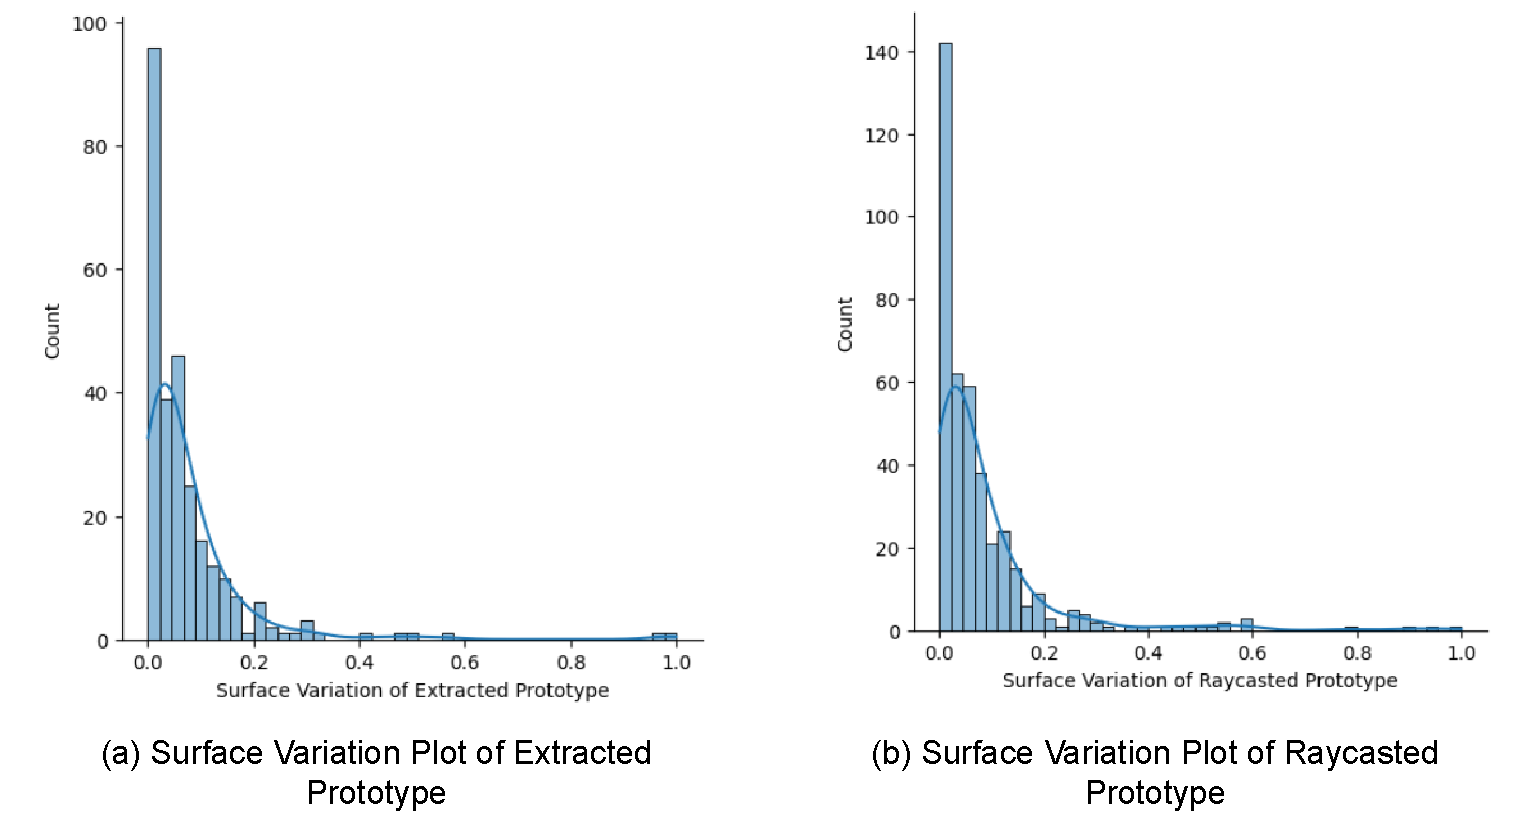
\includegraphics[width=1\linewidth]{97_graphics/evaluation/sv_plots.pdf}
    \caption{Surface Variation plot}
    \label{fig:evaluation-sv_plots}
\end{figure}

For this experiment, a radius of 30cm with a maximum value of the nearest neighbor was taken to be 6 as a parameter to calculate the nearest neighbor using KDTree. Using the formula for surface variation as described in equation \ref{eq:surf_var}, surface variation for each point in the point cloud is calculated. The obtained result is normalized on a scale of 0 to 1 and the corresponding plot is displayed as shown in figure \ref{fig:evaluation-sv_plots}. The figure shows the similarities in geometric features (surface variation )between the two point clouds.


\section{Evaluation of Casted Shadow}
For the evaluation purpose, point cloud representing a "flat" surface was captured from the Carla. This point cloud represents a target scene where we would like to do a shadow casting. A prototype "person" was spawned in some location in the target region without changing the orientation of the lidar sensor and the point cloud was saved. This point cloud corresponds to the source scene cloud. The prototype cloud is to be extracted from the source scene cloud and placed in the target scene cloud. Shadow casting by the prototype is performed on the target cloud and the final point cloud is saved. The prototype person is not transformed in the target scene. The difference between the target cloud and the source scene cloud is the availability of the person and its casted shadow, the rest of the points are similar in both point clouds.

\subsection{Confusion Matrix}
Comparison between the shadow is done by finding the corresponding points between the ground truth shadow and the casted shadow. The nearest neighbor search was done to find the equivalent points in the selected ROI of ground truth shadow and predicted shadow cloud. The radius of the sphere for the neighbor search was taken to be 3 centimeters. If no neighbors were found on the corresponding point cloud within this region, the point was considered to be not found. From the found neighbors, based on some threshold value, the neighbors were filtered. If there exists a neighbor after filtering with some threshold distance, the point was considered to be found on both point clouds. If not, the point was labeled as not found. A confusion matrix is plotted as shown in figure \ref{fig:evaluation_cm}.


\begin{figure}[htbp]
    \centering
    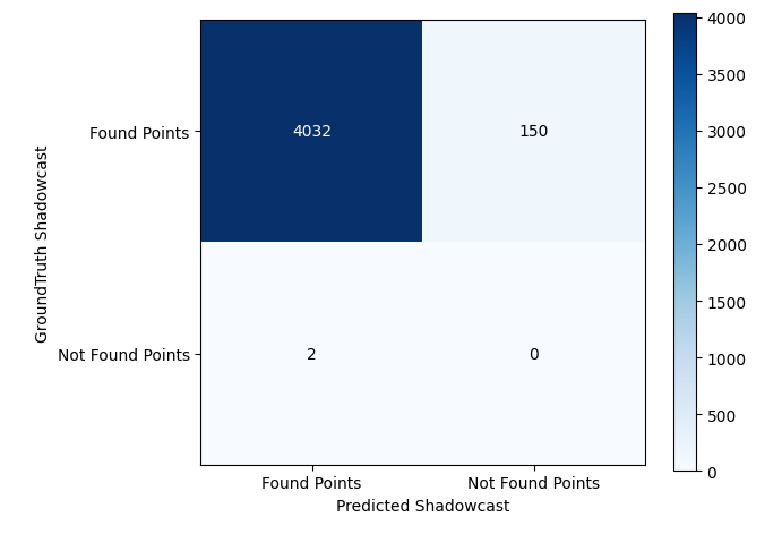
\includegraphics[width=1\linewidth]{97_graphics/evaluation/cm_shadowcast.pdf}
    \caption{Confusion matrix}
    \label{fig:evaluation_cm}
\end{figure}

From the confusion matrix in figure \ref{fig:evaluation_cm}, some observations can be made. Equivalent points for 150 points from the ground truth shadow were not found in the predicted shadow. 2 points available on the predicted shadow cloud were not found in the ground truth shadow cloud. 4032 corresponding points were found in both regions. Unable to say about the points not found on both, the True negative section in the confusion matrix is labeled as 0. From the confusion matrix, the following metrics are observed. 
\begin{itemize}
    \item \textbf{True Positive : }4032
    \item \textbf{True Negative : }0
    \item \textbf{False Positive : }2
    \item \textbf{False Negative : }150
    \item \textbf{Accuracy : }0.963
    \item \textbf{Precision : }0.999
    \item \textbf{Recall : }0.964
    \item \textbf{F1-Score : }0.981
\end{itemize}
The calculation proves that the shadow projection has a high accuracy and a very low error rate. 

Figure \ref{fig:evaluation-distn_betn_corresponding_points_in_shadowcasting} shows the distance between the corresponding points in the predicted shadow cloud and the ground truth shadow cloud. The figure verifies that the points that were considered to be similar in both regions are very similar as the distance between the similar points is in the order of \(1e-9\).

\begin{figure}[htbp]
    \centering
    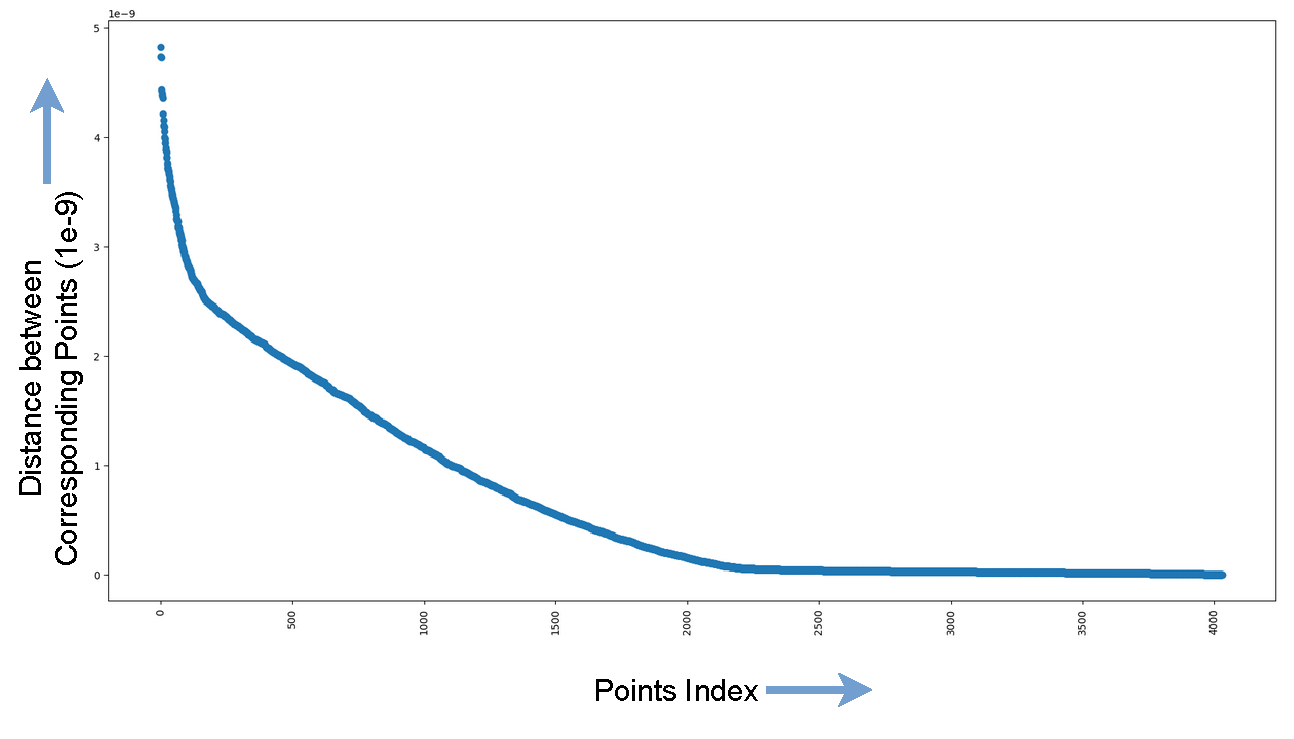
\includegraphics[width=1\linewidth]{97_graphics//evaluation/distn_betn_corresponding_points_in_shadowcasting.pdf}
    \caption{Distance between corresponding points in Shadowcasting}
    \label{fig:evaluation-distn_betn_corresponding_points_in_shadowcasting}
\end{figure}

\subsection{Intersection Over Union}
For the calculation of IOU, the contour points of the shadow region were first extracted for both the point clouds(ground truth shadow and predicted shadow). The extracted 3d-points were projected to the XY plane; i.e. by making the z-value of each point zero. The area of the region occupied by the surface bounding the contour points (i.e. the shadow region) was calculated. The region representing the ground truth shadow and predicted shadow is shown in figure \ref{fig:evaluation-shadow_gt_pred}.
\begin{figure}[htbp]
    \centering
    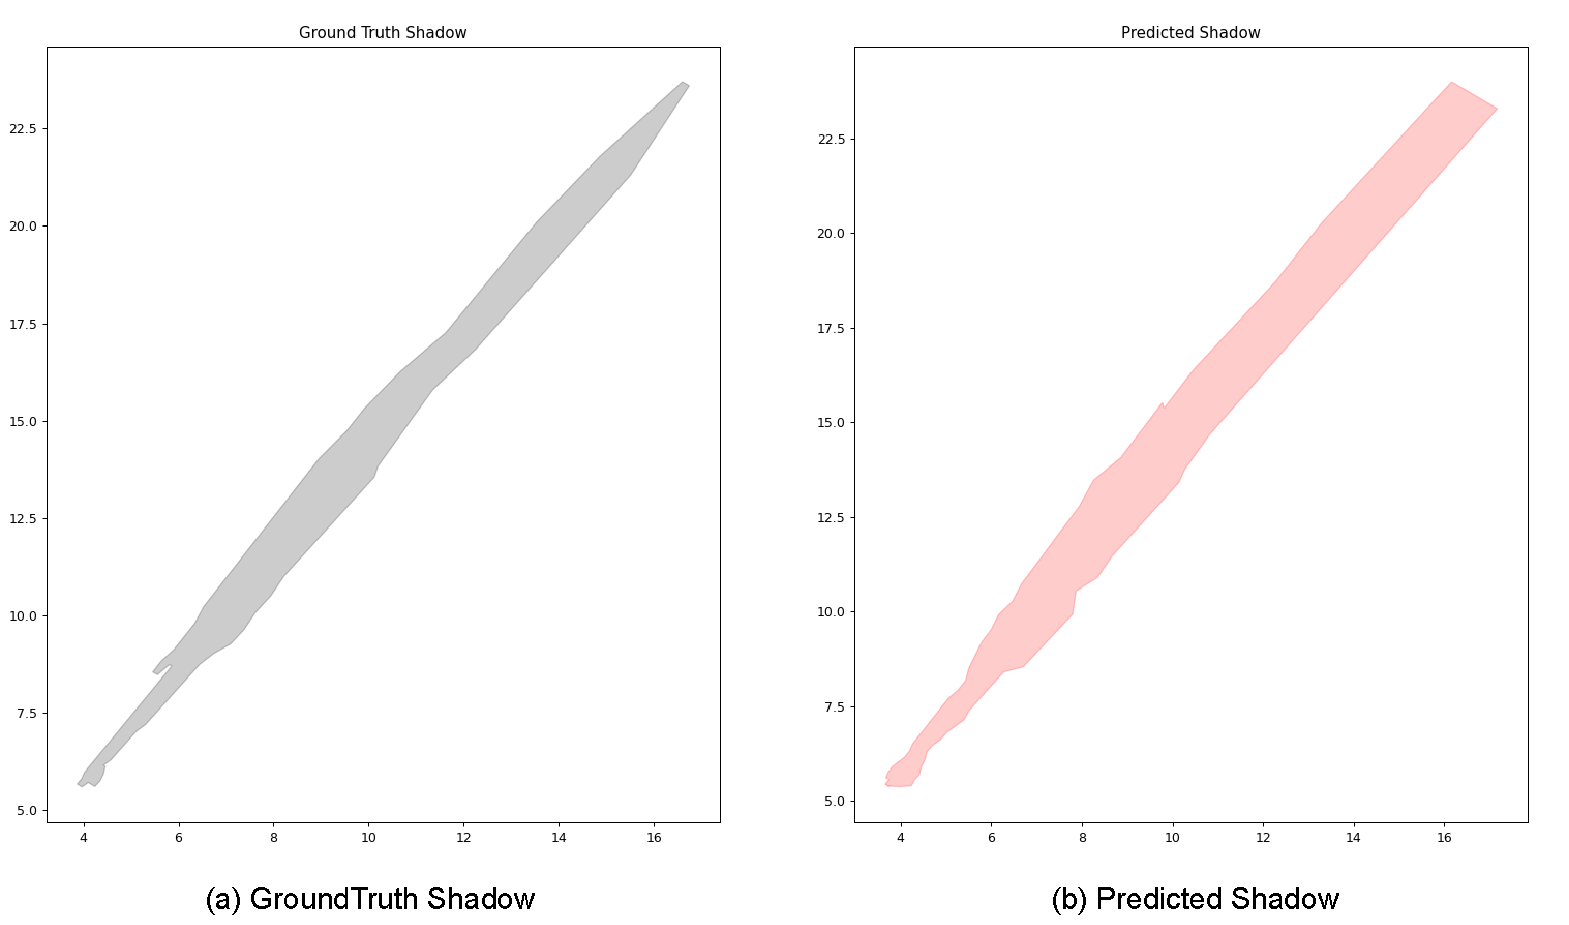
\includegraphics[width=1\linewidth]{97_graphics//evaluation/shadow_gt_pred.pdf}
    \caption{Plot of Ground truth shadow and Predicted Shadow}
    \label{fig:evaluation-shadow_gt_pred}
\end{figure}

Figure \ref{fig:evaluation-shadow_iou} (a) shows the intersection region between the ground truth shadow and predicted shadow by green color. (b) shows the union area between the two regions. Some observations can be made as below. All the observation units (except IOU) are \((m^2)\).
\begin{itemize}
    \item \textbf{Area of Ground Truth Shadow : }17.318
    \item \textbf{Area of Predicted Shadow : }25.886
    \item \textbf{Area of Intersection : }17.293
    \item \textbf{Area of Union : }25.910
    \item \textbf{IOU : }0.667 (Unitless)
    \item \textbf{Area in Ground truth shadow not in Predicted shadow : }0.0248
    \item \textbf{Area in Predicted shadow not in Ground truth shadow : }8.592
\end{itemize}

\begin{figure}[htbp]
    \centering
    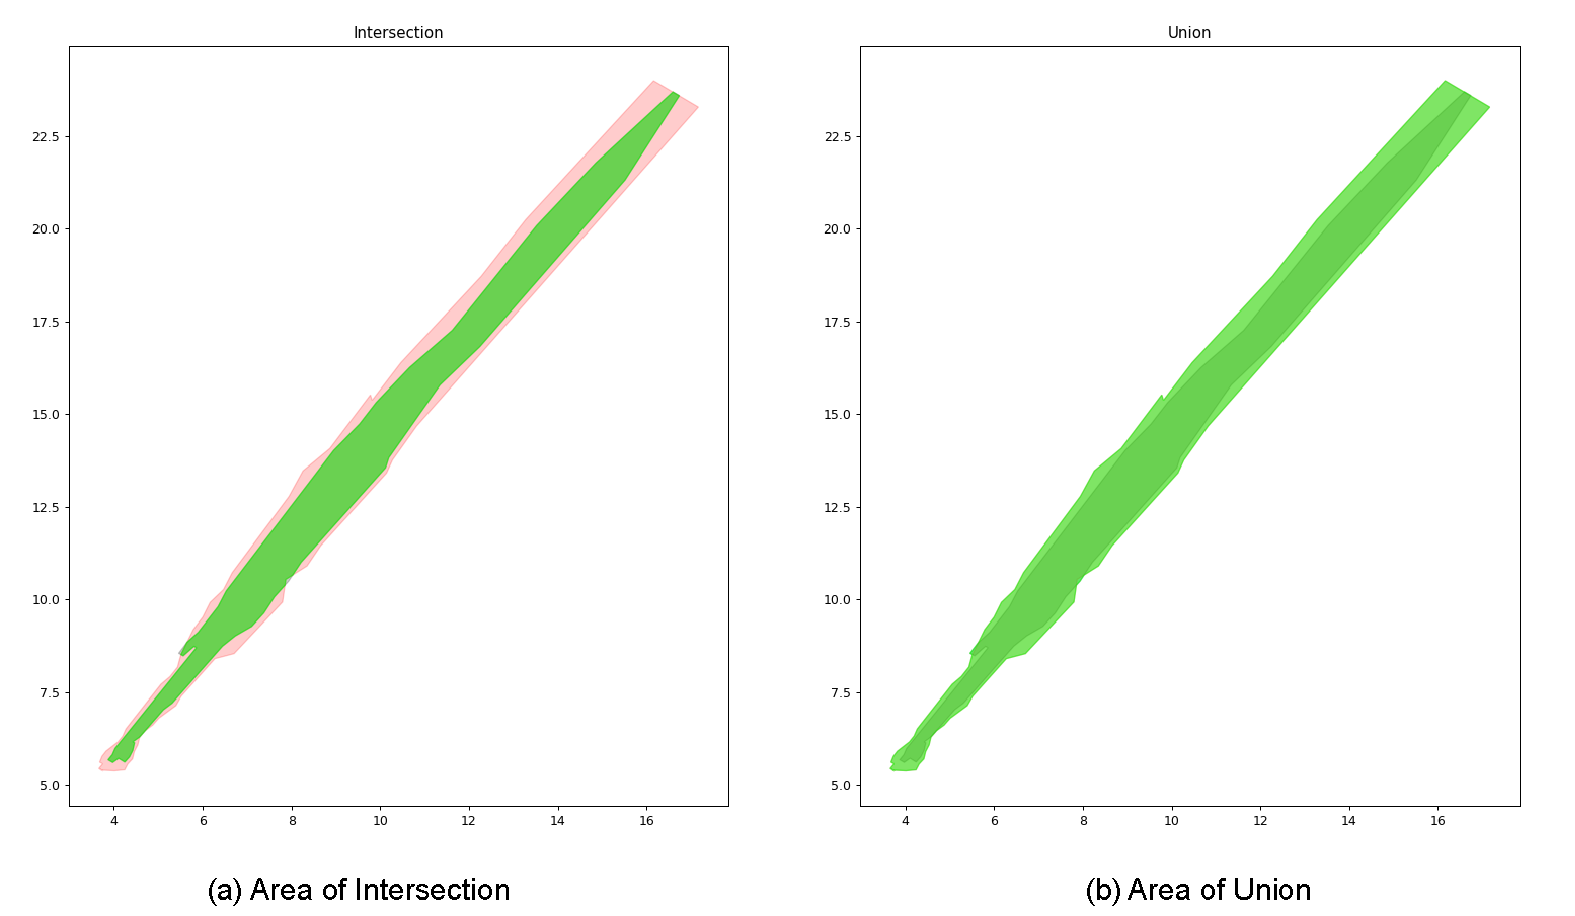
\includegraphics[width=1\linewidth]{97_graphics//evaluation/shadow_iou.pdf}
    \caption{Intersection and Union between the ground truth shadow region and predicted shadow region plot}
    \label{fig:evaluation-shadow_iou}
\end{figure}

It can be observed from the findings about the accuracy of ground truth shadow. All the ground truth shadow region was predicted. The IOU score was 0.667. It can be improved if the reconstructed surface would accurately represents the extracted prototype. 

